\chapter{Mapping Functions for SDOG and the Extension Method} \label{chap:mapping}
The previous two chapters reported methods for creating hierarchical grid geometry to be used in a 3D DGGS.
However, grid geometry on its own is not sufficient for functioning as a DGGS.
Geospatial data, which represent locations on a globe reference, need to be mapped to the domain of the grid system and vice versa.
In a 2D DGGS, this is handled by the projection method and its inverse.
A projection $P$ maps the surface of a sphere or ellipsoid (reference domain) to the grid domain; the inverse $P^{-1}$ does the opposite.
A 3D DGGS requires a similar operation but instead maps the volume of a ball (reference domain) to some other volume (grid domain).
We refer to these mapping functions by $M$ to distinguish them from their 2D projection counterparts.


Since our modifications of SDOG have the same grid domain as the reference space, such mappings are not strictly required; despite this, they can still be useful.
As we will explore in \cref{chap:coding}, the regularity of midpoint refinement in SDOG allows for efficient encoding and decoding algorithms---this is not the case for our modifications.
However, a mapping between conventional SDOG and the modified grids allows for efficient encoding and decoding to be done with the conventional grid, with inputs and outputs converted between the two representations.


On the other hand, for 3D DGGS's resulting from the extension of a polyhedron-based 2D DGGS, the grid domain is not the same as the reference one.
For these grids, such mappings are necessary.
Beyond their necessity, though, these mappings also allow for other properties of the grid system to be achieved. Most notably, volume preservation can be improved with appropriate mapping functions.


\begin{figure}[ht!]
	\centering
	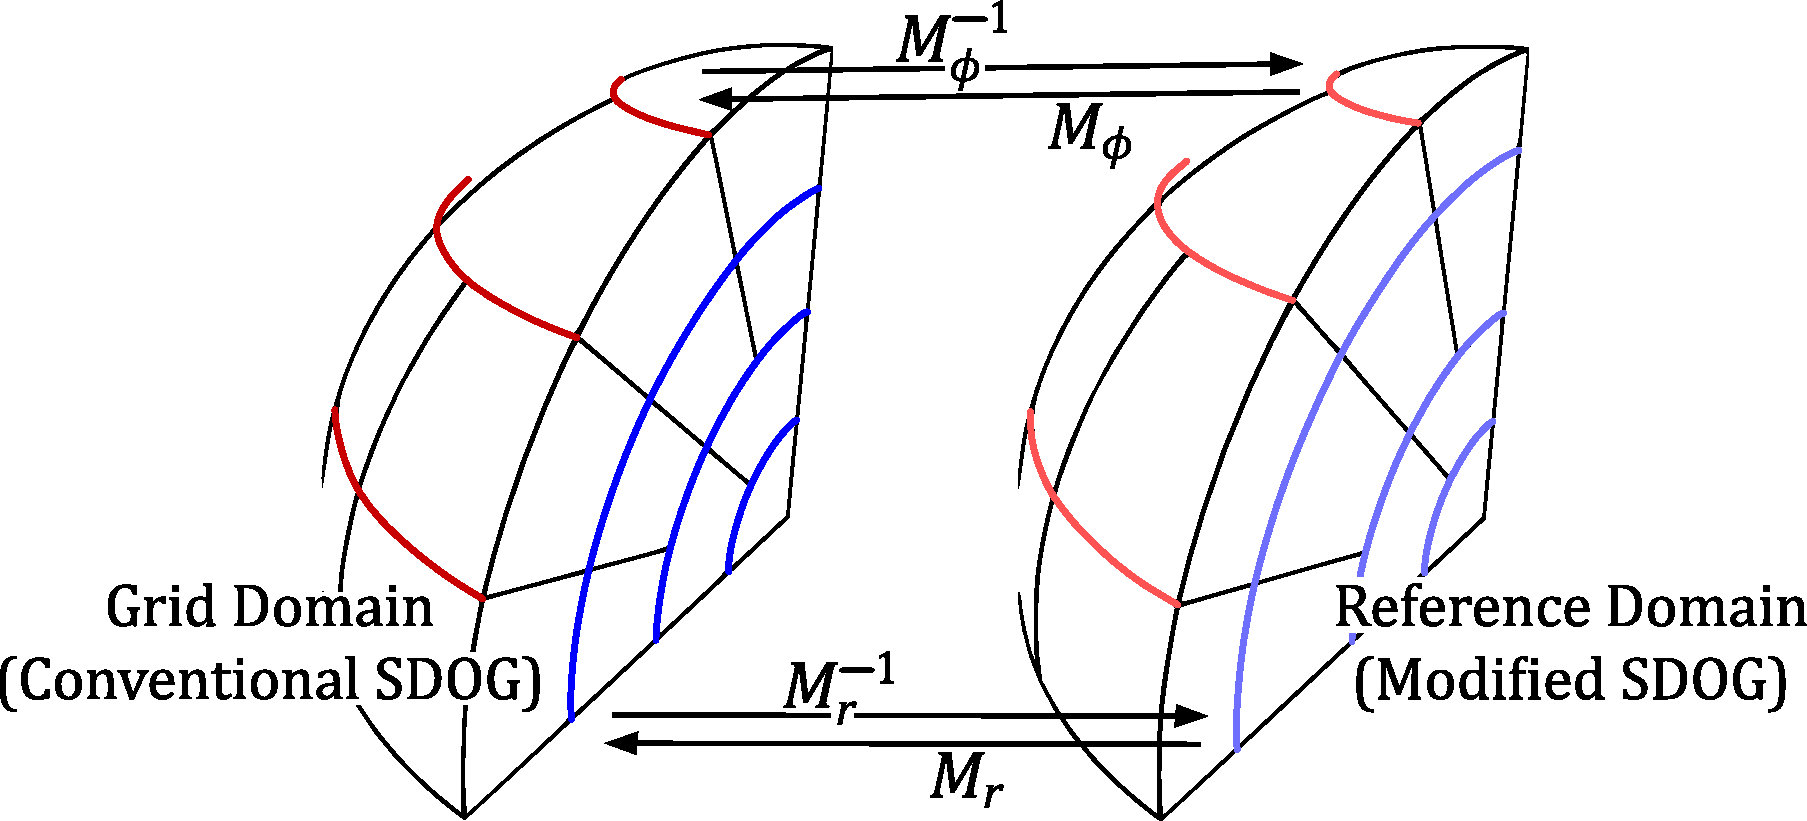
\includegraphics[width=0.77340\textwidth]{map-overview-sdog.pdf}
	\caption[Title]{
		Caption go here
	}
	\label{fig:map-overview-sdog}
\end{figure}


\begin{figure}[ht!]
	\centering
	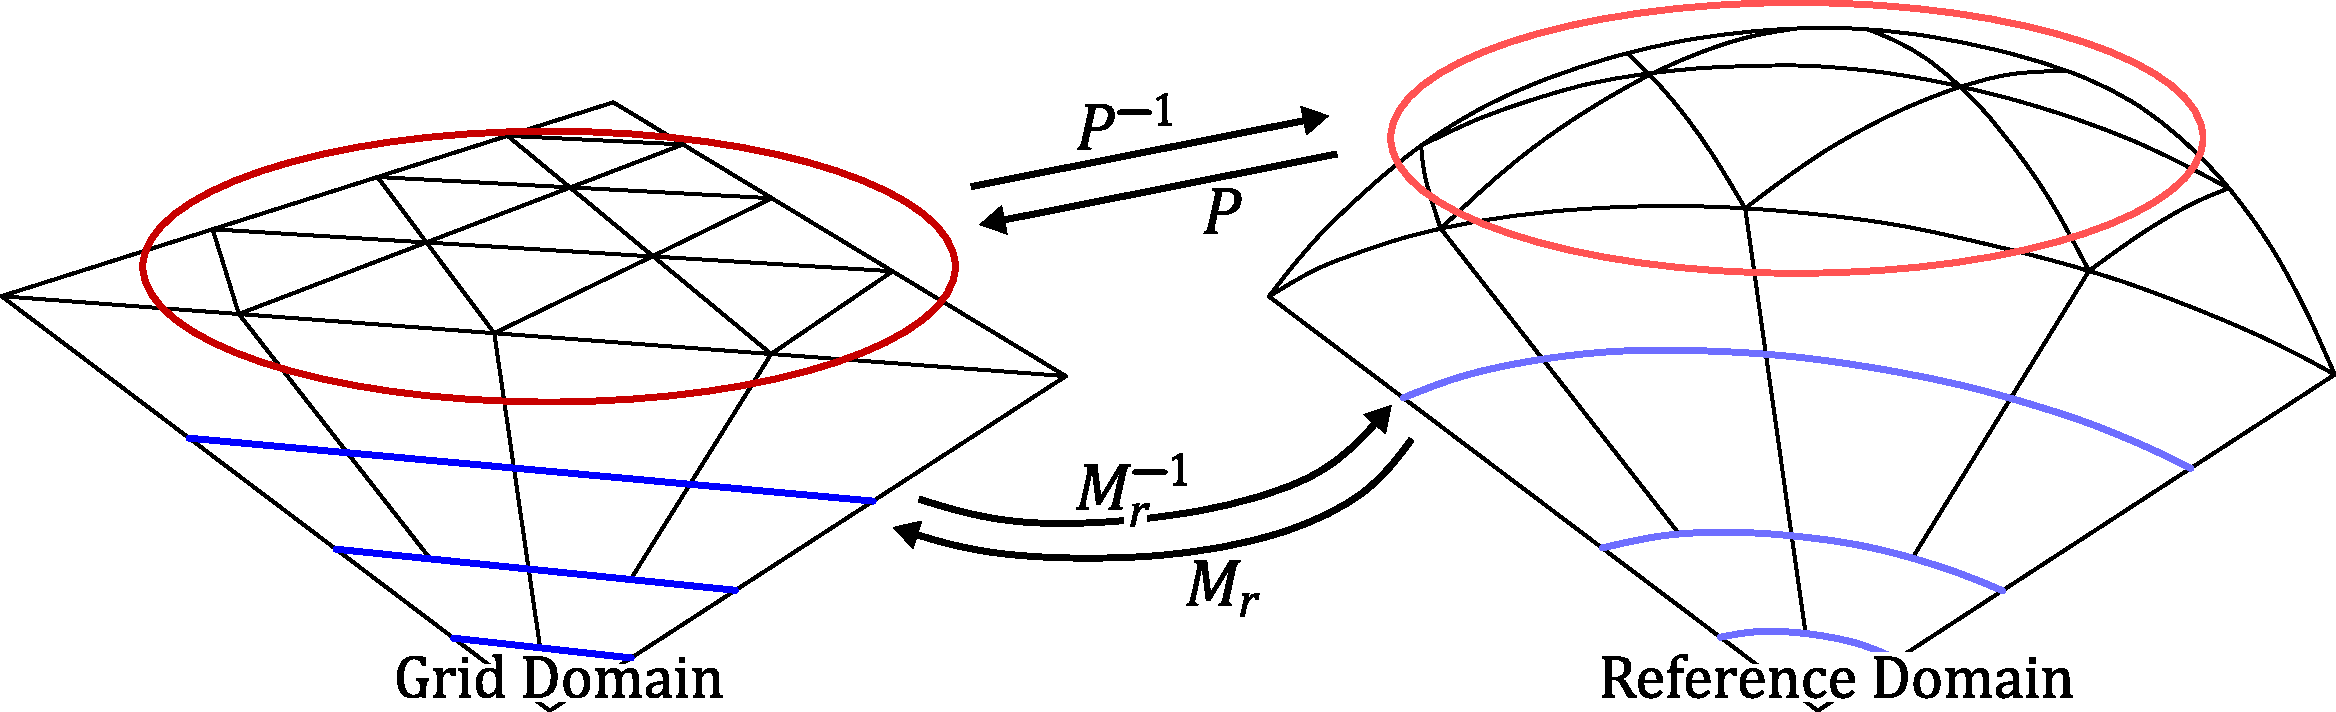
\includegraphics[width=\textwidth]{map-overview-prism.pdf}
	\caption[Title]{
		Caption go here
	}
	\label{fig:map-overview-prism}
\end{figure}


In this chapter, we present two sets of mapping functions for use with our SDOG modifications and grid extension method:
the first is a set of radial mappings used for both approaches;
the second is a set of latitude mappings for SDOG, which operate on similar principles as the radial ones.
An overview of how we use these functions with the SDOG modifications and grid extension method is demonstrated in \cref{X,Y}, respectively.
We do not provide mappings for the surface coordinates in the grid extension method, as the projection scheme of the input DGGS is responsible for this.
We present the inverse mappings first, as the geometric intuition for the role of these operations is more apparent than the forward.
For SDOG, the inverse takes conventional SDOG and maps it to the modified grids presented in \cref{chap:sdog}.
For the grid extension method, the inverse takes the prismatoid grid and maps it to the corresponding grid in reference space.
We then derive the forward mappings from the inverses.


This chapter consolidates similar mapping functions presented in our \textit{Geoinformatica}~\cite{ulmer2020toward} and \textit{IJGI}~\cite{ulmer2020general} articles.
The exact derivations and formulations are modified, but the core principles and results are the same.


\section{Mapping Functions} \label{chap:6:functions}
The mapping functions for semiregular degenerate refinement have two primary objectives: shift the boundaries of the regular regions of the grid and warp the interiors of these regions.
\Cref{fig:mapping} demonstrates how we accomplish this for a generic semiregular degenerate refinement grid when mapping a point.
The boundaries of the regular region that contain a point are first determined in both the grid and reference domains.
A parameterization function then parameterizes the location of the point relative to the two boundaries in its current domain, and an interpolation function converts said parameter into a location in the other domain.
Below, we derive these parameterization and interpolation functions for the radial and latitudinal coordinate mappings.


\begin{figure}[ht!]
	\centering
	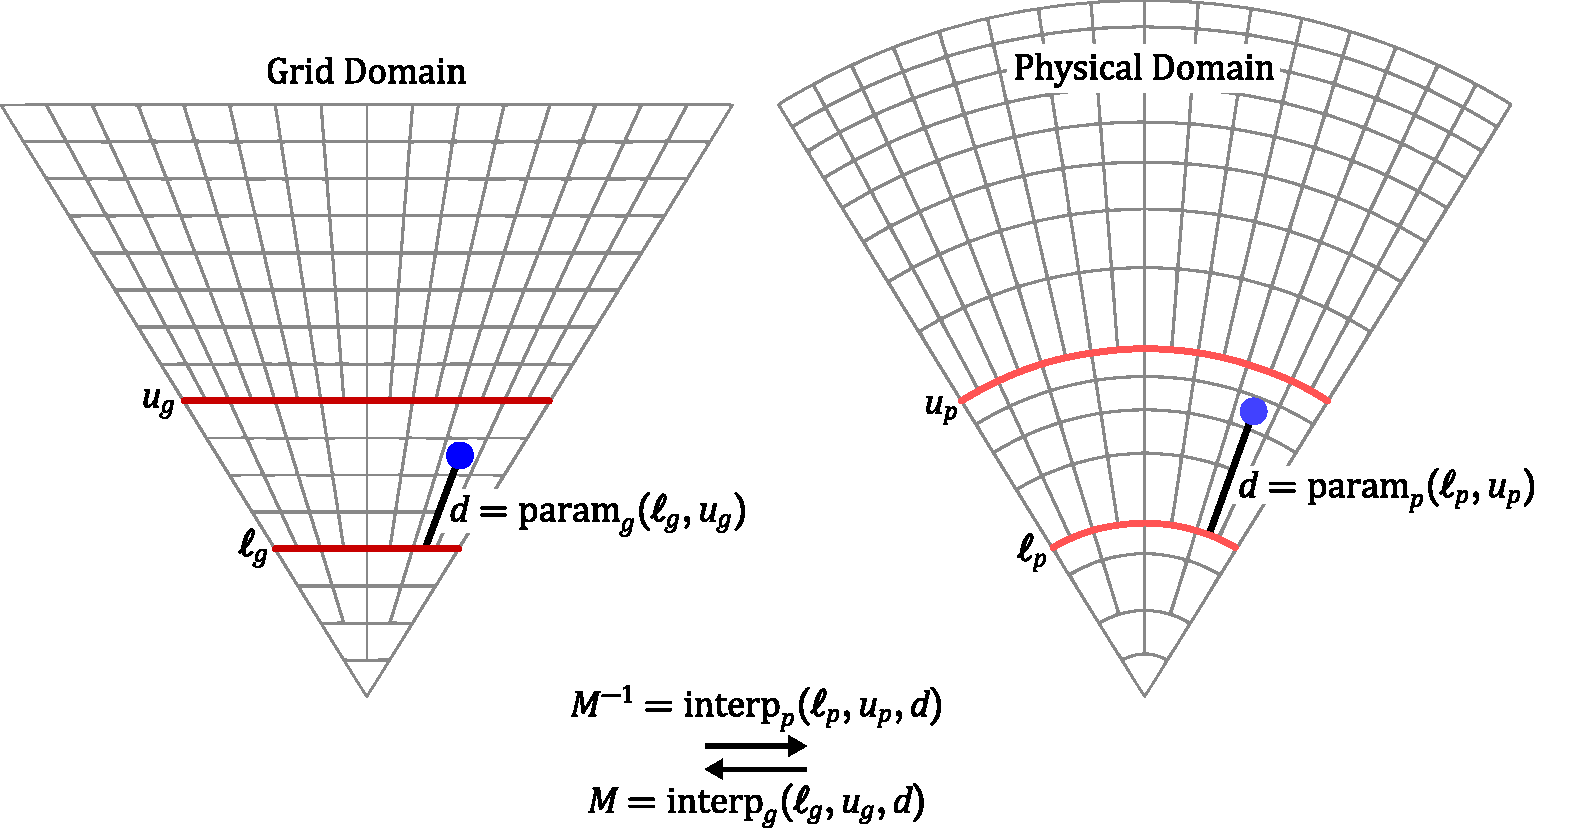
\includegraphics[width=\textwidth]{mapping.pdf}
	\caption[Overview of mapping for semiregular degenerate refinement grids]{
		Overview of the general mapping technique we use for a semiregular degenerate refinement grid.
		The upper and lower values of the regular region containing the point are first calculated in both domains.
		The point is then parameterized between these two values in the appropriate space (reference for forward, grid for inverse).
		Finally, an interpolation function converts this parameter into a value in the other domain (grid for forward, reference for inverse)
	}
	\label{fig:mapping}
\end{figure}


\subsection{Radial Mappings} \label{chap:6:radial}
Our goal is to define a function $M_r(r)$ that maps a reference radius to a radius in the grid domain.
Consider radius to be normalized with $\hat{r} = r / R_\mathrm{max}$.
Also, recall that for the grid extension method, a radius in the grid domain is defined as the radius of the polyhedron's circumscribing sphere.


We first note the similarities and differences between SDOG and the grid extension method in the radial dimension.
Referring back to \cref{fig:sdog-shells} for SDOG and comparing it to \cref{fig:prismatoid-shells} for the extension method, we see radial splits have the same effect and structure.
Therefore, in comparing the volume of shells, \cref{eq:shellVolume} also holds for the grid extension method.
However, the refinement factor for the extension method is not always 1:8, as it depends on the surface refinement factor; thus, the best placement for the split is not necessarily $\alpha = 1/2$.
Instead, we want $\alpha^3 = 1 / f^{\ 3}$ (where $f$ is once again the 1D refinement factor) which is satisfied when $\alpha = 1/f$.
Therefore, the SDOG mappings will be a special case of the extension ones where $f = 2$.
We derive the general mappings below in terms of $\alpha$, starting with the inverse mappings.


\begin{figure}[ht!]
	\centering
	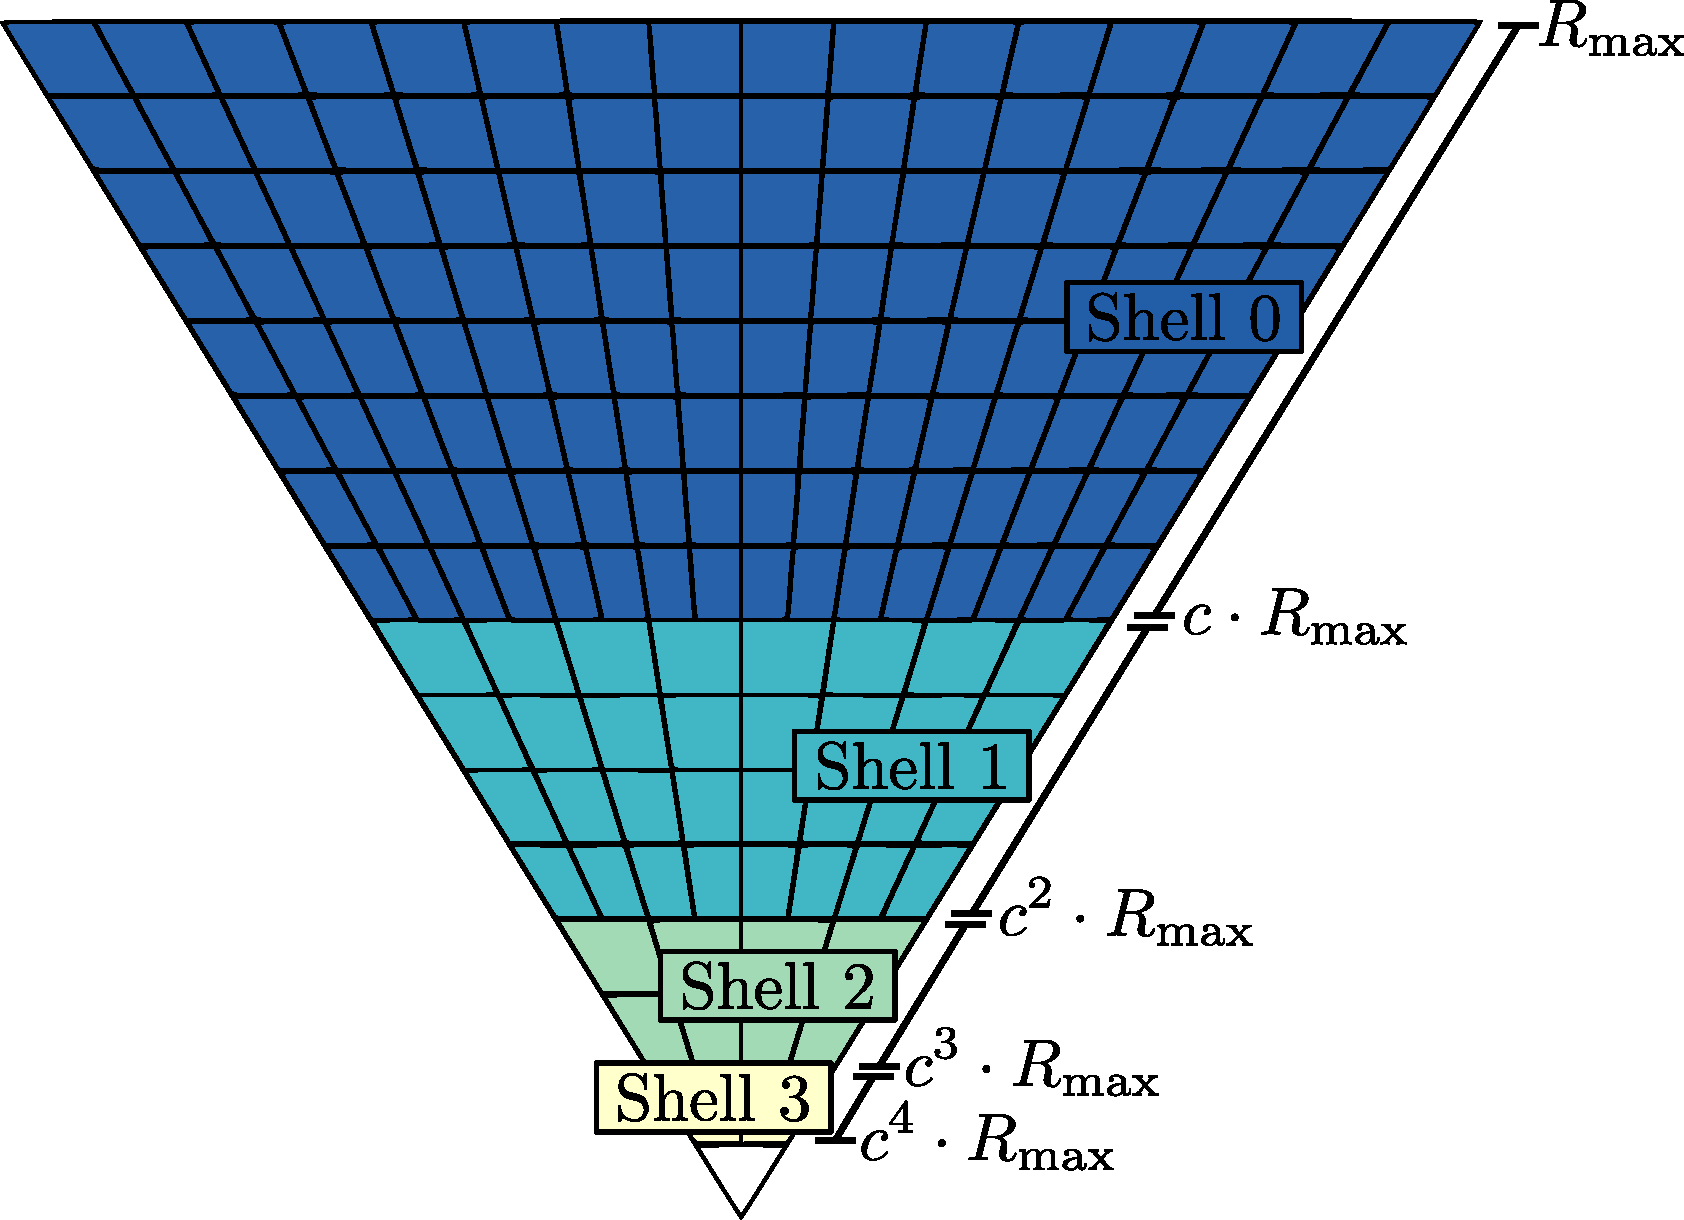
\includegraphics[width=0.675\textwidth]{prismatoid-shells.pdf}
	\caption[Spherical shells that result from the grid extension method]{
		Radial splits of central layers divide the grid into regions that represent spherical shells.
		At $k$ levels of refinement there are $k$ shells and the central layer.
		These shells are similar and should have a mapped volume proportional to the number of cells they contain
	}
	\label{fig:prismatoid-shells}
\end{figure}

In order to achieve the desired results of the mapping, radii at powers of $1/2$ in grid space should be mapped to corresponding powers of $\alpha$ in the reference domain.
For a given value of $\hat{r}$ in the grid domain, we need to find the appropriate powers that bound the point.
Looking at \cref{fig:sdog-shells,fig:prismatoid-shells}, we see these are simply the shell number and shell number plus one for the upper and lower, respectively.
The shell that contains $\hat{r}$ is given by $s = \lfloor \log_{0.5} \hat{r} \rfloor$.
Therefore, the actual radii in both reference and grid space are obtained by raising $\alpha$ and $0.5$ to these powers.
We use $\ell$ to refer to the lower value and $u$ the upper one---subscripts $g$ and $r$ refer to the grid and reference domain, respectively.
Thus,
%
\begin{equation*}
\ell_r = \alpha^{s + 1}, \quad u_r = \alpha^s, \quad \ell_g = 0.5^{s + 1}, \quad \text{and} \quad u_g = 0.5^s.
\end{equation*}
%

We now need to find the appropriate parameterization and interpolation functions for the mapping.
Since radial splits are spaced uniformly in the grid domain, we use a linear parameterization
%
\begin{equation} \label{eq:radialInvD}
d = \frac{ \hat{r} - \ell_g }{ u_g - \ell_g }.
\end{equation}
%
For the interpolation function, how $d$ is interpolated between $\ell_r$ and $u_r$ affects volume preservation.
To obtain the different SDOG modificaitons, we generalize \cref{eq:radBlend} to get
%
\begin{equation} \label{eq:radialInv}
M_r^{-1}(\hat{r}) = \sqrt[t]{ d u_r^{t} + \left( 1 - d \right) \ell_r^{t} }.
\end{equation}
%


Now, we derive the forward mapping by inverting the inverse.
Inverting the interpolation functions gives the corresponding parameterization function, and vice versa.
Solving \cref{eq:radialInv} for $d$ gives us
%
\begin{equation} \label{eq:radialForwD}
d = \frac{ \hat{r}^{\,t} - \ell_r^{\,t} }{ u_r^{\,t} - \ell_r^{\,t} }
\end{equation}
%
and solving \cref{eq:radialInvD} for $\hat{r}$ yields
%
\begin{equation} \label{eq:radialForw}
M_r (\hat{r}) = d u_g + \left( 1 - d \right) \ell_g.
\end{equation}
%
The values of $\ell$ and $u$ are calculated the same as the inverse, but the shell is now $s = \lfloor \log_{c} \hat{r} \rfloor$.
Note that the output of both \cref{eq:radialInv,eq:radialForw} are normalized and must be multiplied by $R_\mathrm{max}$ for the true radii.


\begin{figure}[ht!]
	\centering
	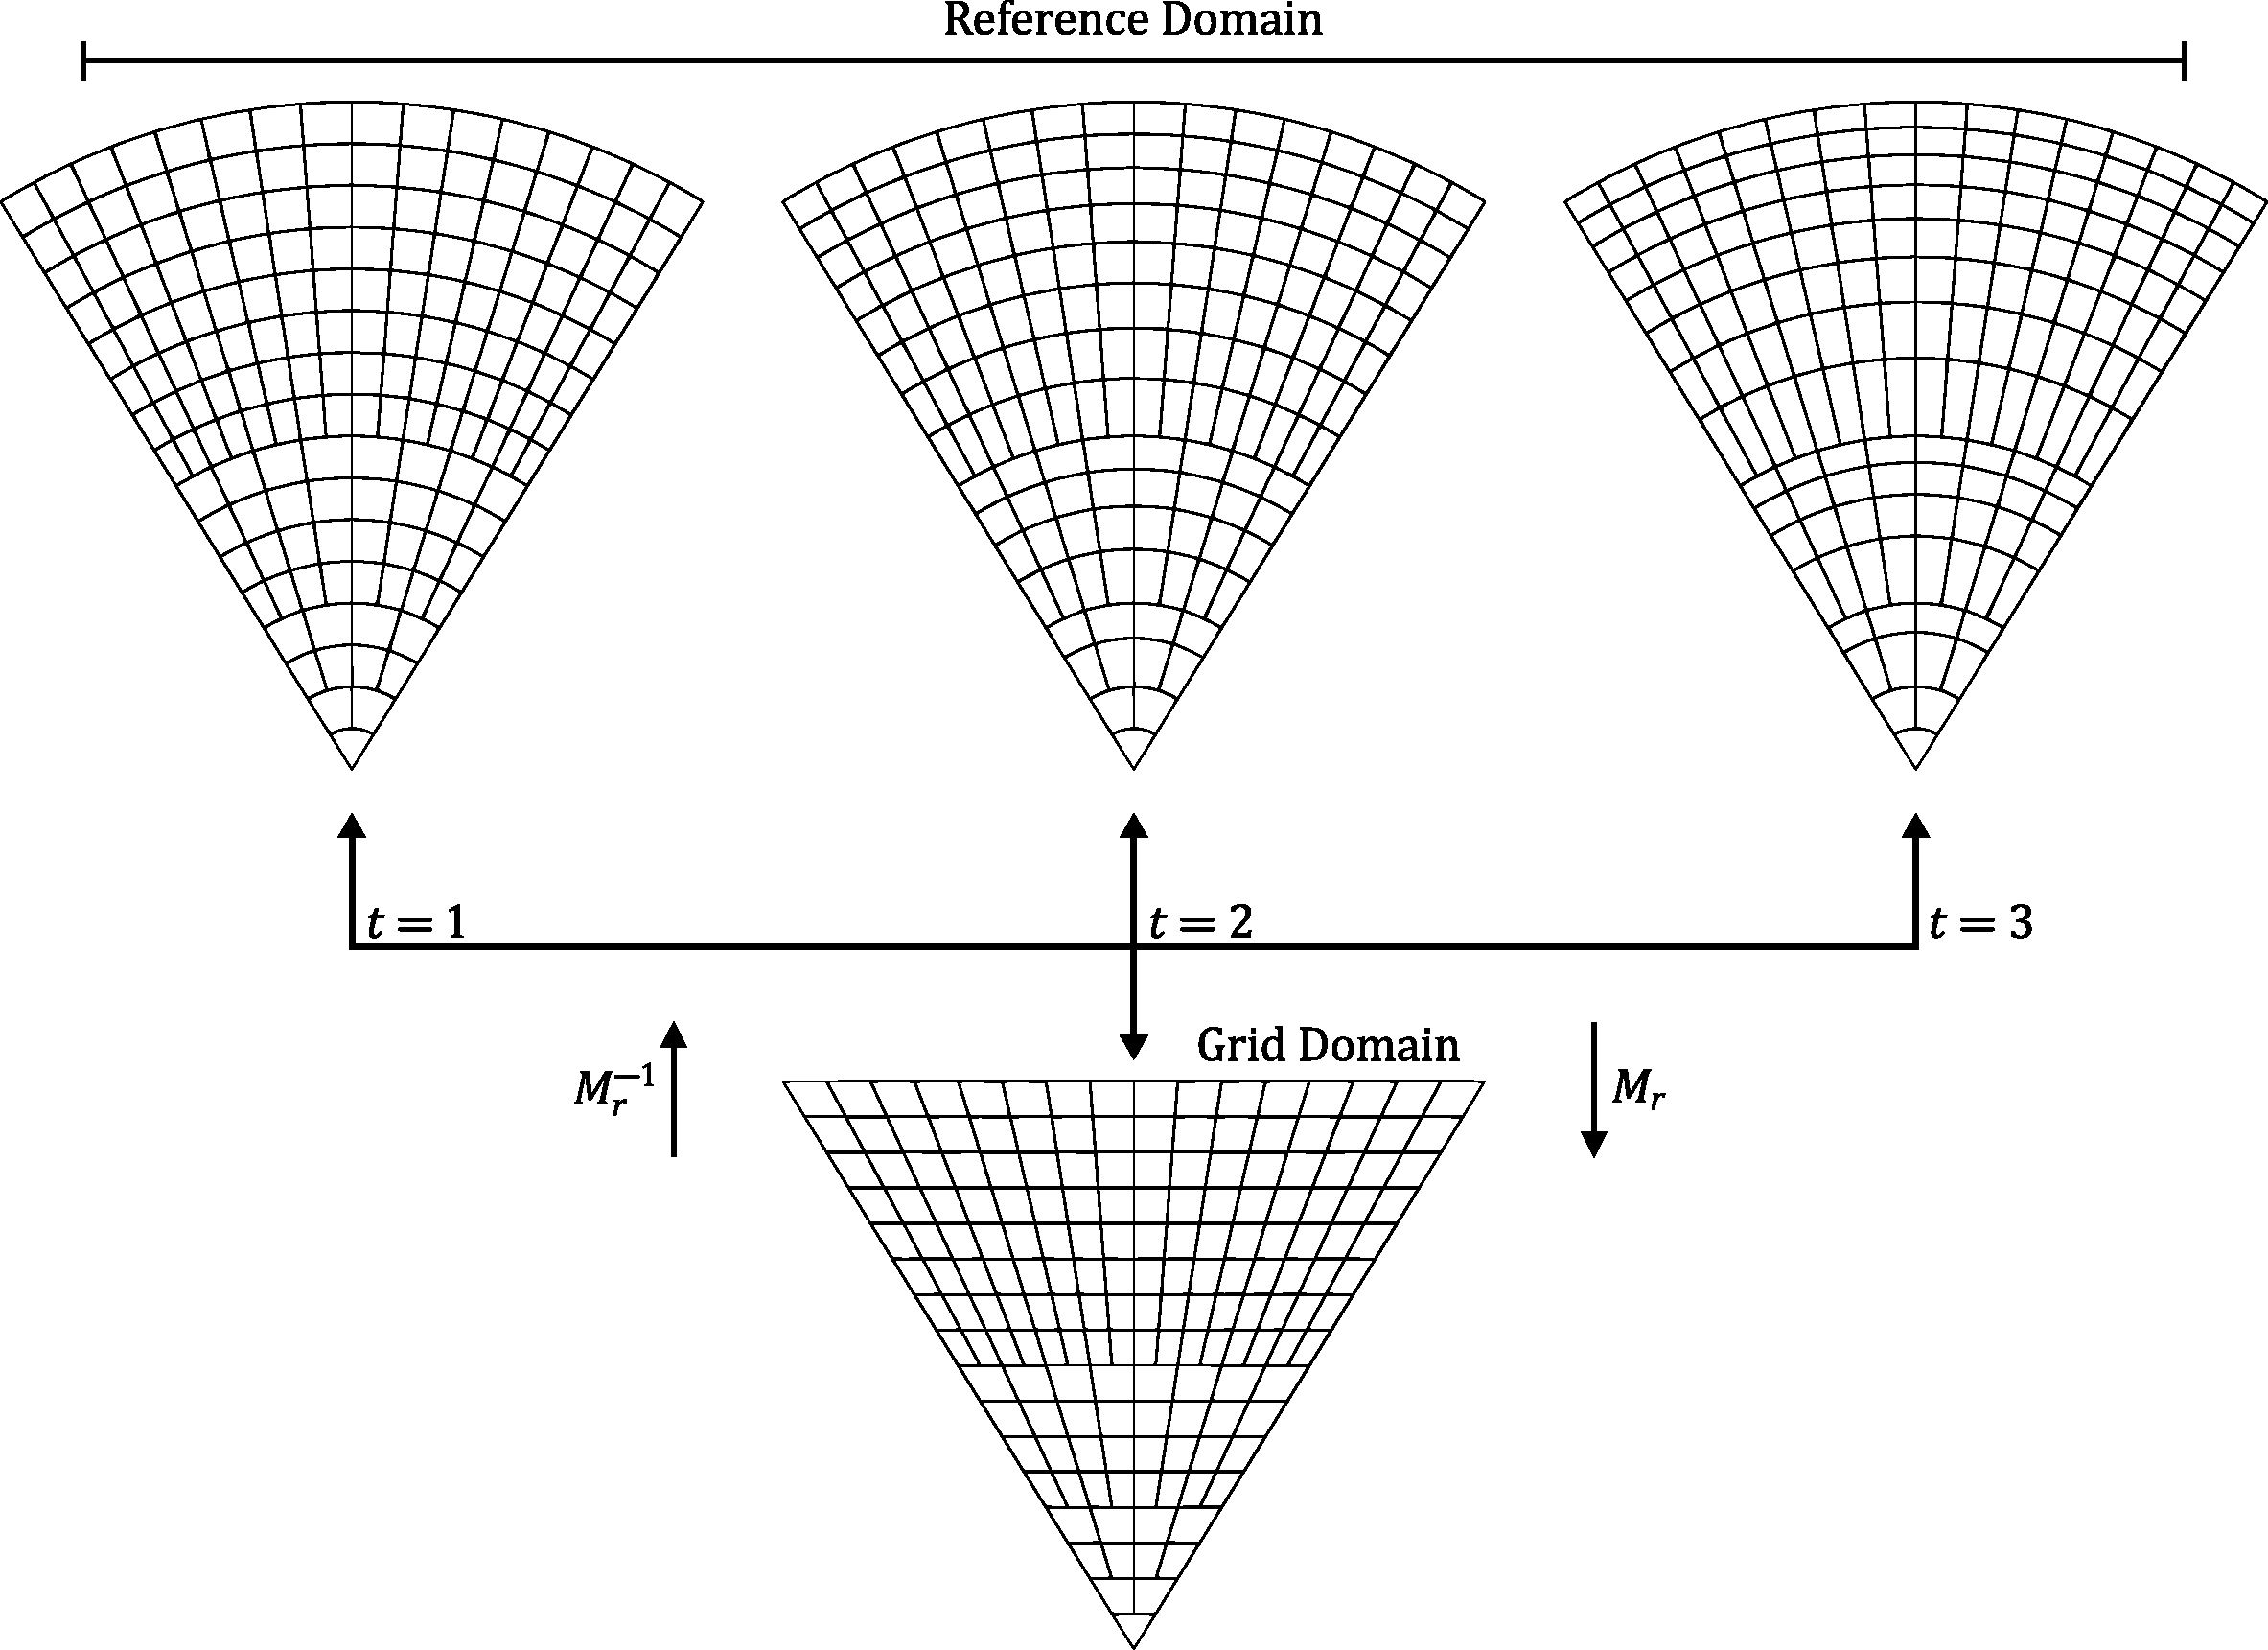
\includegraphics[width=\textwidth]{prismatoid-mappings.pdf}
	\caption[Radial mappings applied to the grid extension method]{
		Radial mappings with different values of $t$---along with a normalization polyhedral projection---applied to a prismatoid grid resulting from the grid extension method.
		Just as with the modified SDOG refinements, cells are stretched and squashed to preserve volume with the effect increasing with $t$
	}
	\label{fig:prismatoid-mappings}
\end{figure}


The results of this mapping for different values of $t$ applied to the grid extension method are shown in \cref{fig:prismatoid-mappings}.
Generally speaking, the value of $t$ has the same effect for the grid extension method as for SDOG, blending between compactness and volume preservation.
Setting $t=1$ ensures that each shell has volume proportional to the number of cells it contains; however, it does little to preserve volume and keeps cells as compact as possible.
When $t=3$, all cells in the same shell have perfect volume preservation assuming the input DGGS is \textit{area} preserving.
Depending on the layering sequence, however, volume will not necessarily be preserved between cells in different shells.
Additionally, just as with SG and LG cells in SDOG, the central layer will never have volume preservation with the others.


For the grid extension method, these mappings also have the side effect of changing the aspect ratio of cells in grid space as compared to in reference space.
Therefore, when determining the refinement parameters needed to achieve the desired aspect ratio, we should consider the cells in reference space as opposed to grid space.
We accomplish this by setting the value of $\nu$ in \cref{eq:extraSplits,eq:extraSurface} to be $(1 - \alpha)$.


\subsection{Latitude Mappings for SDOG} \label{chap:6:latitude}
While the grid extension method only requires a radial mapping, our SDOG modifications also modify latitude splitting surfaces.
Therefore, a set of latitude mappings is also required.
Just as with the radial mappings, our goal is to define a function $M_\varphi(\varphi)$ that maps a reference latitude to one in the grid domain. Likewise, we consider latitude to be normalized with $\hat{\varphi} = \pm (2\varphi) / \pi$, where the sign is equal to the sign of the latitude.


The derivation follows the same steps as the radial mappings.
Referencing \cref{fig:sdog-zones}, zones increase with increasing latitude as opposed to shells which increase with \textit{decreasing} radius.
Thus, the zone that contains $\hat{\varphi}$ is $z = \lfloor \log_{0.5} ( 1 - \hat{\varphi} ) \rfloor$.
We then calculate values of $\ell$ and $u$ just as with the radial mapping but accounting for the opposite direction.
Additionally, for the reference domain values, these are the sine of angles as opposed to angles themselves, since \cref{eq:latVol} operates on the sine of angles.
The final values are then
%
\begin{equation*}
\ell_r = 1 - 0.25^{z}, \quad u_r = 1 - 0.25^{z + 1}, \quad \ell_g = 1 - 0.5^z, \quad \text{and} \quad u_g = 1 - 0.5^{z + 1}.
\end{equation*}
%

Again, we now need to find the appropriate parameterization and interpolation functions for the mapping.
Since latitude splits are also spaced uniformly in the grid domain, we once again use a linear parameterization
%
\begin{equation} \label{eq:latInvD}
d = \frac{ \hat{\varphi} - \ell_g }{ u_g - \ell_g }.
\end{equation}
%qgi

Similarly, for the interpolation function, how $d$ is interpolated between $\ell_r$ and $u_r$ affects volume preservation.
To obtain the different SDOG modificaitons, we generalize \cref{eq:latBlend} to get
%
\begin{equation} \label{eq:latInv}
M_\varphi^{-1}(\hat{\varphi}) = h \arcsin \left( d \sin \left( \frac{1}{h} \arcsin u_r \right) + \left( 1 - d \right) \sin \left( \frac{1}{h} \arcsin \ell_r \right) \right).
\end{equation}
%
This simplifies to
%
\begin{equation*}
M_\varphi^{-1}(\hat{\varphi}) = d \arcsin u_r  + \left( 1 - d \right) \arcsin \ell_r
\end{equation*}
%
for the latitude method as $h \rightarrow \infty$ and
%
\begin{equation*}
M_\varphi^{-1}(\hat{\varphi}) = \arcsin \left( d u_r + \left( 1 - d \right) \ell_r \right)
\end{equation*}
%
for the volume method when $h = 1$.
The volume method is most efficient (one arcsin), the latitude one less so (two arcsins), and the balanced the worst (three arcsins, two sins).


Once again, we derive the forward mapping by inverting the inverse.
Solving \cref{eq:latInv} for $d$ yields
%
\begin{equation} \label{latForwD}
d = \frac{ \sin \left( \frac{1}{h} \hat{\varphi} \right) - \sin \left( \frac{1}{h} \arcsin \ell_r \right) }{ \sin \left( \frac{1}{h} \arcsin u_r \right) - \sin \left( \frac{1}{h} \arcsin \ell_r \right) }
\end{equation}
%
and solving \cref{eq:latInvD} for $\hat{\varphi}$ provides
%
\begin{equation} \label{eq:latForw}
M_\varphi (\hat{\varphi}) = d u_g + \left( 1 - d \right) \ell_g
\end{equation}
%
The values of $\ell$ and $u$ are the calculated the same as the inverse, but the zone is now $z = \lfloor \log_{0.25} ( 1 - \sin \hat{\varphi} ) \rfloor$.
Just as with the radial mappings, the output of \cref{eq:latInv,eq:latForw} are normalized and must be multiplied by $\pm \pi / 2$ for the true latitudes.


\Cref{latForwD} simplifies to
%
\begin{equation*}
d = \frac{ \hat{\varphi} - \arcsin \ell_r }{ \arcsin u_r - \arcsin \ell_r}
\end{equation*}
%
for the latitude method as $h \rightarrow \infty$ and
%
\begin{equation*}
d = \frac{ \sin \hat{\varphi} - \ell_r }{ u_r - \ell_r }
\end{equation*}
%
for the volume method when $h = 1$.
Just as with the inverse, the volume method is most efficient (one sin), the latitude one less so (three arcsins), and balanced one the worst (three arcsins, four sins).


\section{Summary}
The use of mapping functions allows for geospatial data---which represent physical locations---to be located within the domain of a 3D DGGS.
This operation is necessary for encoding and decoding data.
Furthermore, these mappings allow for achieving properties such as volume preservation in the resulting grid system.
This chapter provides two similar sets of mapping functions that operate independently from each other on radius and latitude, respectively.
Both the forward and the inverse of the functions provided are closed-form (no iterative solves) and operate in constant time regardless of the inputs.
Efficiency for the latitude mapping varies significantly on the level of volume preservation desired, which is a result of the blending function chosen in \cref{chap:4:balanced}.
We explore the efficiency of these mappings more in the next chapter.
